% ARCHIVE ONLY. Consolidated and revised in appendix.tex on 2026-09-23.
% Not included by main.tex. Edit appendix.tex for the current manuscript.
\section{Additional Mathematical Analyses}
\label{app:additional_math}
The following elementary results connect window-level observations to two limits of prefix control. They are exact under the stated assumptions, not empirical claims or proposed changes to the frozen algorithm.

\subsection{When can later windows still change the vote?}
Let $c_a$ count all valid votes for answer $a$ already generated, including votes from rejected windows. Let $\ell$ be a unique current leader and let $r$ be an upper bound on the number of answers still to be generated. Include an unseen competitor with count zero when defining $c_{(2)}=\max_{a\ne\ell}c_a$. Each remaining trajectory supplies at most one unit vote, and earlier votes cannot be removed or reweighted.

\begin{proposition}[Irreversible plurality]
\label{prop:lock}
If $c_\ell-c_{(2)}>r$, then $\ell$ is the unique final plurality winner for every possible continuation, including adaptive and dependent continuations. If $c_\ell-c_{(2)}<r$, a continuation assigning every remaining vote to a strongest competitor can overturn the leader. At equality a competitor can tie, so the outcome depends on the fixed tie rule.
\end{proposition}
\begin{proof}
For any competitor, the largest possible increase in its count relative to the leader is $r$. Thus its final deficit is at least $c_\ell-c_a-r$. A strictly positive minimum guarantees the leader remains unique. Conversely, giving all $r$ votes to a strongest competitor realizes that maximum increase, proving the remaining statements. Invalid outputs can only reduce the number of added votes and cannot break the sufficient condition.
\end{proof}

The statement concerns the realized vote, not correctness. Once a wrong leader is locked, a rollback cannot repair the final answer under this aggregation rule. Once a correct leader is locked, later prefixes cannot change final correctness either. For a fixed $B=32,m=4$, one may test the sufficient condition after window $j$ using $r=32-4j$. This is a deterministic diagnostic, not the heuristic margin-$2$ rule and not a new stopping controller in the reported experiments. The condition says only that later votes cannot alter the outcome; it does not undo any effect of earlier prefixes on the current counts.

There is also a useful consequence for Theorem~\ref{thm:decomposition}. On a locked history, $V^S$ is constant over all admissible next windows, so $d_j(h)=0$. Accordingly,
\[
 |A_P-A_S|\leq\min\left\{1,\sum_j\E_P\left[
 \ind\{H_j\text{ is not locked}\}\,
 \TV(K_j^P(\cdot\mid H_j),K_j^S(\cdot\mid H_j))\right]\right\}.
\]
This refinement localizes possible final-vote effects to histories where future votes can still matter. It does not assert that unlocked histories are recoverable under the model's actual support, nor that their increments are favorable.

\subsection{Higher marginal correctness can yield a worse majority}
For a binary illustration, condition on a history with $n$ earlier votes, $k$ of them correct, and $r=B-n$ remaining votes. A random shared prefix $Z$ induces a correctness probability $p_Z$; conditional on $Z$ and the history, the remaining answers are independent Bernoulli variables. With ties counted as failures, let $t=\lfloor B/2\rfloor+1-k$. Using the binomial tail from Equation~\ref{eq:exactbinary}, the conditional final success probability is
\begin{equation}
 A_{\mathrm{shared}}(h)=\E[Q_r(p_Z,t)\mid h].
 \label{eq:mixturevote}
\end{equation}
If an independent prefix were instead drawn for each remaining answer under this stylized model, the probability would be $Q_r(\bar p,t)$, where $\bar p=\E[p_Z\mid h]$. These two expressions generally differ even at identical marginal correctness. Independent-prefix resampling here is an analytical comparator, not an evaluated path-consistency variant.

\begin{proposition}[Curvature of the voting response]
For $1\leq t\leq r$ and $0<p<1$,
\[
 \frac{d Q_r(p,t)}{dp}
 =r\binom{r-1}{t-1}p^{t-1}(1-p)^{r-t},
\]
and the sign of its second derivative is the sign of
$(t-1)-(r-1)p$. Thus $Q_r$ is concave above $p=(t-1)/(r-1)$ and convex below it when $r>1$. If the support of $p_Z$ lies wholly in the concave region, sharing cannot improve the voting probability relative to independent resampling at the same mean; in the convex region the inequality reverses.
\end{proposition}
\begin{proof}
Differentiate the finite binomial sum. Adjacent terms cancel, leaving the stated first derivative. Its logarithmic derivative is $(t-1)/p-(r-t)/(1-p)$, which has the stated sign. Jensen's inequality on either curvature region gives the comparison. For $r=1$ the response is linear. For $t\leq0$ or $t>r$ it is constant. When the support crosses the inflection point, these local curvature statements imply no universal ordering.
\end{proof}

For a finite-budget counterexample retaining the root votes, take four independent root answers with correctness probability 0.6 and 28 later answers sharing a latent prefix. Independently of the root, let $p_Z=1$ with probability 0.65 and $p_Z=0$ otherwise. The final vote is correct exactly when $p_Z=1$, hence its accuracy is 0.65. In contrast, 32 independent answers with correctness probability 0.6 succeed with probability $Q_{32}(0.6,17)=0.835203095$. Every later answer in the shared construction has higher marginal correctness (0.65 versus 0.6), and the mean across all 32 is 0.64375, yet its majority is worse. This deliberately extreme mixture is not a fitted path-consistency model or an assertion that these prefixes occur in the experiments. It demonstrates why per-trajectory correctness and agreement alone do not identify the accuracy of a shared-prefix vote.

\section{Llama Modern-Benchmark Results}
\label{app:llama}
These completed Llama-3.1-8B-Instruct runs use the same $B=32,m=4,C=0.8$ algorithmic budget, with chat prompting and an 8,192-token limit. They are separated from the thinking-model main table, not excluded from the evidence.
\begin{table}[htbp]
\centering\small
\caption{Additional Llama results. Accuracy is in percent; token costs are per-question means.}
\begin{tabular}{llrrrrrr}
\toprule
Model & Dataset & Pass@1 & SC & PC & SC tok & PC tok & Save \%\\
\midrule
\inputrows{tables/llama_modern_rows.tex}
\bottomrule
\end{tabular}
\end{table}
Llama/MATH-500 has 333/500 correct for both methods (including ten credited engineering items) with 8.3\% fewer tokens. Only one AIME 2024 question uses a nonempty prefix. None does on AIME 2025, where both methods have zero correct final answers. On GPQA-D, path-consistency drops from 82 to 78 correct (2.02 percentage points), with 5.3\% fewer tokens. These results delimit the main-model findings: agreement-based reuse does not supply reasoning ability when useful early trajectories are absent.

\section{Window-Level Measurement Details}
\label{app:windows}
\paragraph{Final outcomes by path-consistency behavior.}
\begin{table}[htbp]
\centering\small
\caption{Final outcomes by observed PC behavior on Llama/GSM8K. Each row compares SC and PC on the same questions. Gains/losses are paired correctness changes; savings use the ratio of total tokens within the row. Groups are defined after generation and are not randomized treatments.}
\label{tab:behavior}
\begin{tabular}{lrrrrr}
\toprule
PC behavior & Questions & SC correct & PC correct & Gains/losses & Save \%\\
\midrule
\inputrows{tables/behavior_rows.tex}
\bottomrule
\end{tabular}
\end{table}

The 1,120 questions using prefixes without rollback account for the largest saving (48.3\%), but also six losses and no gains. The 101 questions with rollback have three gains and two losses, and save 14.6\%. The remaining 98 questions never use a prefix and exactly match self-consistency. The favorable net change within the rollback group does not estimate a causal rollback benefit: difficulty and generated history determine group membership. Likewise, stable agreement does not certify a safe prefix.

All statistics use the four complete Llama/GSM8K shards underlying Table~\ref{tab:composition}. Every question has exactly eight windows of four traces. At window $j$, cumulative accuracy uses the final aggregation rule on the first $4j$ traces, retaining invalid-answer handling and first-occurrence tie breaking. It does not use the controller's selectively admitted answer set. The eighth-window reconstruction is checked against every stored final correctness flag. The first window is checked for paired-root agreement.
\begin{table}[htbp]
\centering\small
\caption{Exact window counts and mean costs on 1,319 questions. Use and rollback are counts of questions in that window. Prefix length includes zeros and counts the one shared prefix; SC/PC tokens sum the four new continuations. Final two columns count cumulative correct votes.}
\begin{tabular}{rrrrrrrr}
\toprule
Window & Use & Prefix tok & Rollback & SC tok & PC tok & SC correct & PC correct\\
\midrule
\inputrows{tables/window_rows.tex}
\bottomrule
\end{tabular}
\end{table}
The behavior groups partition questions by whether any window used a nonempty prefix and, if so, whether any logged decision includes rollback. They do not classify whether the prefix was semantically correct. Group savings are ratios of token totals rather than unweighted averages of per-question saving percentages. The rollback group contains 129 rollback windows on 101 questions. Its three gains and two losses cannot establish what those same questions would have done with recovery disabled. No independent-repetition error bars are inferred from these single-run curves.

\section{Ablation Protocols and Remaining Controls}
\label{app:ablation_design}
\paragraph{Status and shared controls.}
The source-selection and recovery experiment in Section~\ref{sec:ablations} is complete for one run of each arm on DeepSeek-V4-Flash/MATH-500. The second main-text ablation reports compiled agreement-threshold results on DeepSeek-V4-Flash/GSM8K. The completed matched-history prefix-length intervention on MATH-500 is retained as a supplementary analysis. These ablations do not overwrite the default main-table runs. Correctness annotations are evaluation-only and never enter prefix control.

\paragraph{Source selection and recovery.}
The four arms are BLC/recovery, uniform/recovery, BLC/no-recovery, and uniform/no-recovery. Uniform selection uses the same eligible source pool and a recorded selection seed. The eligibility, answer masking, prefix-length grid, and generation settings are unchanged. With recovery enabled, the controller uses trial, commitment, single-level rollback, and disabling after two consecutive failures. With recovery disabled, failures are still detected and excluded from the admitted control/source pool, but the active failed prefix is retained and the consecutive-failure reset is disabled. A retained trial can later commit if it passes validation. This tests the recovery mechanism as a whole, not stack popping in isolation. All valid completed answers remain in the final vote.

The four arms share 490 evaluated questions and the same self-consistency roots. Accuracy counts ten held-out engineering items as correct, so the reported correct counts are 438, 436, 433, and 433 out of 500. Relative to the default arm, the other arms have paired gains/losses of 3/5, 4/9, and 5/10. Exact two-sided McNemar tests for these comparisons all have $p>0.1$. The interaction in evaluated correct counts is $423-426-423+428=2$, not evidence of compounded damage when both components are removed.

The numbers of proposals with nonfinite selected-source scores are 731/1,899, 1,009/1,897, 757/1,869, and 1,002/1,853, respectively. These counts are not the fraction of candidate pools with fully observed scores. Additional independently seeded repetitions and uncertainty estimates for the interaction remain future work. An incorrect modal answer is defined relative to the evaluation reference, not by a step-level proof that its entire source prefix is wrong.

\subsection{Agreement-threshold protocol}
\label{app:threshold}
Table~\ref{tab:threshold} uses the compiled records for all 1,319 GSM8K questions. At $C=0$, the self-consistency and path-consistency correct counts are 1,283/1,280; at $C=0.7$, they are 1,282/1,281; at $C=0.8$, they are 1,277/1,277. Accuracy uses the format-tolerant regrade. The self-consistency pools come from separate API runs, so each row retains its own self-consistency reference rather than using a single baseline to calculate differences. The $C=1.0$ endpoint reproduces the self-consistency reference for $C=0.8$. The $C=0$ arm retains source eligibility, feasible-prefix requirements, and the remaining controller rules.

The $C=0.8$ record combines regraded accuracy from the original paired shards with token costs from the vote-v2 run that reuses their self-consistency roots. The $C=0$ and $C=0.7$ records use the earlier voting keys. These provenance differences are retained in the compiled comparison and prevent attributing cross-row differences solely to $C$. No API timing comparison or cross-version incorrect-promotion comparison is used to establish a threshold effect.

The table retains the prior default $C=0.8$ without selecting a test-set winner. Additional repetitions are needed to assess run-to-run variability. Lower thresholds relax the gate at a fixed history, but do not imply a monotonic closed-loop accuracy or cost trend. Threshold selection for a new application uses separate validation data and a prespecified accuracy tolerance and budget, not the GSM8K test comparison.

\subsection{Supplementary matched-history prefix-length intervention}
\label{app:length_intervention}
The completed experiment fixes the first-window history and BLC-selected source from the reference run. It includes 466 questions with common support across all five levels. Of the 24 exclusions, 19 fail the gate and five lack a feasible endpoint. The target population is therefore the gate-passing, common-support subset, not all MATH-500 questions. Questions are not selected by their correctness.

For each included question, the run completed eight repetitions at each of $r\in\{0,0.2,0.4,0.6,0.8\}$, generating a window of four answers, for 18,640 intervention units. The final-vote diagnostic retains the original four root answers and 24 cached unprefixed self-consistency answers, replacing only the intervened window. Holding the cached continuation fixed pairs the comparisons across levels, but does not integrate over fresh self-consistency continuations. Accordingly, the current diagnostic is conditional on the cached continuation and must not be equated with the full expectation defining $d_j(h)$ in Equation~\ref{eq:risk}. Conditional resampling of the remaining horizon and increasing the repetition count are possible extensions, not completed measurements.

Analyses must preserve question-level pairing and distinguish repetition variability from question-to-question variability. The resulting prefix-length analysis is not a test-time controller and does not select a threshold from test results.

\paragraph{Secondary controls.}
Window-size sweeps are separate from the main-text threshold ablation; window index in Figure~\ref{fig:windows} must not be relabeled as a window-size ablation. Fixed stopping schedules isolate continuation shortening in AC/ESC composition. Cache-on/off and prefill/decode measurements separate serving effects. These controls belong in the appendix unless their results materially change the main explanation. None chooses $C^\star$ from a test set or replaces the fixed length grid with a PVC lookup policy.

\section{Historical Motivation and Its Interpretation}
\label{app:motivation}
The earlier manuscript's characterization experiment partitions self-consistency-generated tokens according to whether the completed trajectory has a correct final answer. That statistic describes token allocation after outcomes are known. It does not establish the fraction of compute that could be safely removed at generation time: incorrect samples can still be informative for estimating an answer distribution. Similar-looking intermediate steps also need not be interchangeable reasoning states.

\begin{figure}[htbp]
\centering
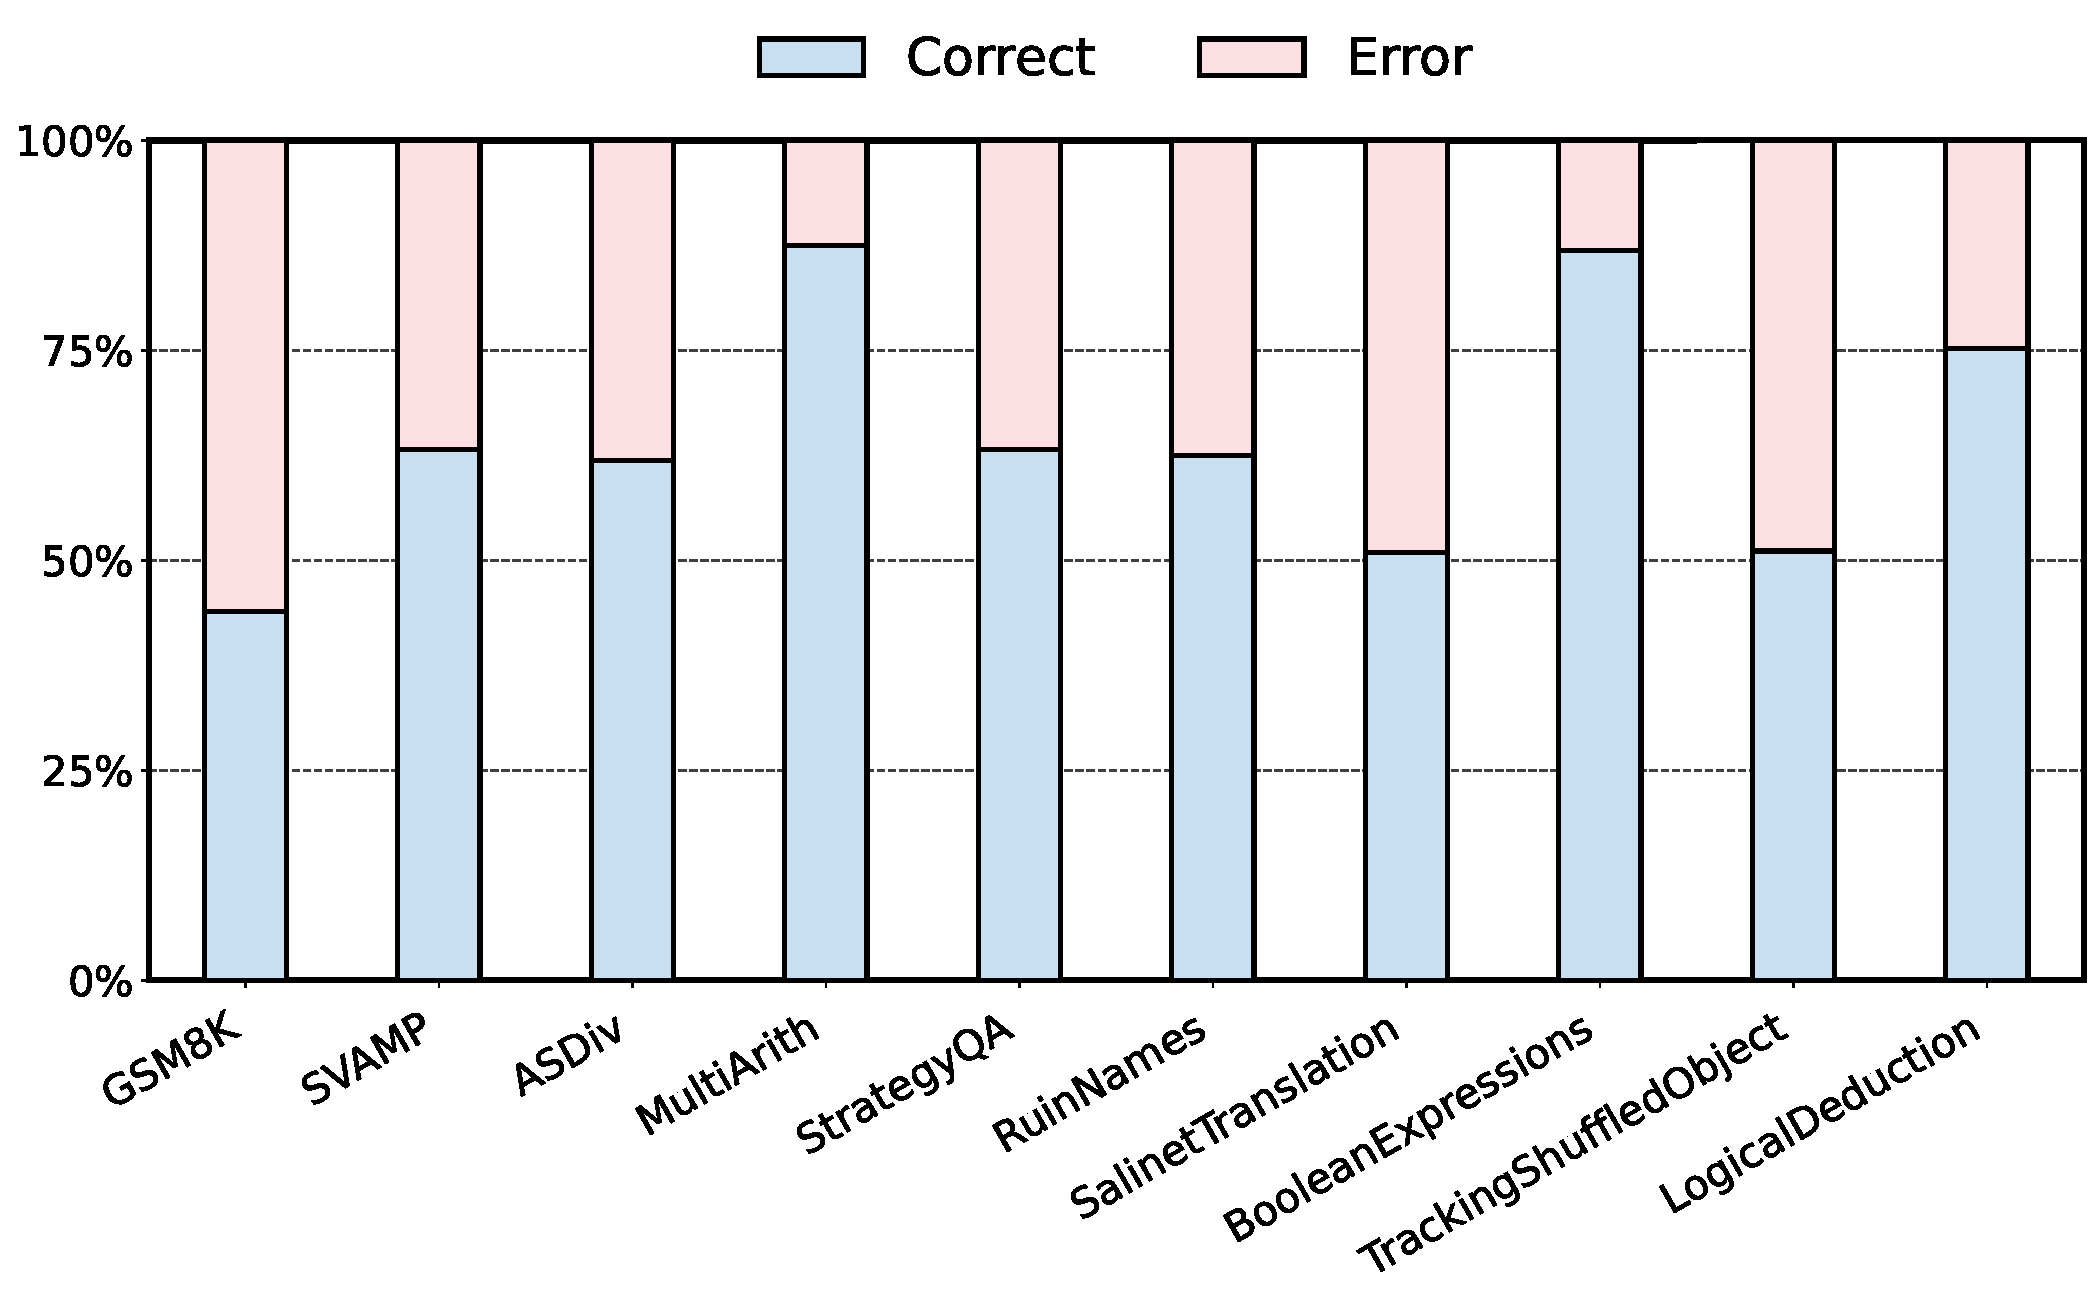
\includegraphics[width=0.85\linewidth]{figures/historical_characterization.pdf}
\caption{Historical SC token allocation, reproduced unchanged from the earlier manuscript's characterization figure. ``Error'' labels tokens on trajectories with incorrect final answers, not tokens proved unnecessary. This is archival evidence: its generating model/budget metadata and raw counts have not been independently reconstructed for this revision. It is not a $B=32$ main-protocol result.}
\label{fig:historical_motivation}
\end{figure}
The historical characterization figure is retained only in Figure~\ref{fig:historical_motivation}; its numerical bars are not transcribed into the new protocol's tables or presented as a fresh measurement. The supplementary intervention in Appendix~\ref{app:length_intervention} examines how prefix length, continuation correctness, and generation cost change under an identical early history. Its scope is conditional on selected histories and a cached continuation. It does not establish that tokens on incorrect trajectories can safely be removed.
